\chapter{实现}
\label{cha:impl}

\section{性能模型}
\label{sec:impl_model}
    我们建立性能模型的主要方法是,单独对某个操作进行测试,得到该操作在不同参数下的运行时间。然后通过对运行时间数据进行分析,建立性能模型。
    
    我们的实验平台如下:
    
    \begin{itemize}
        \setlength{\itemindent}{1em}
        \item CPU:2个8核Intel Xeon CPU(E5-2620 v4)
        \item RAM:256GB
        \item GPU:4块Nvidia GPU(Tesla V100),使用NVLink连接
        \item OS:Ubuntu 18.04.1 LTS
    \end{itemize}

    CPU上的数据通过两种方式来获得。第一种是对TensorFlow的会话执行进行计时。这种方式的问题在于会计入图处理等额外时间,带来误差。另一种方式是使用TensorFlow Profiler获得执行的流程,在跟踪数据中直接拿到操作的运行时间。但是这种方式的坏处在于,如果数据规模较小,操作被优化了,或是调用了其他函数进行执行,那么在跟踪数据中不会出现这一部分的运行时间。我们的测试主要通过第一种方式进行,因为通常这种额外时间比较短,不会影响到我们的预测,而第二种方式会缺省大量数据,也导致我们无法对小规模数据建模。

    GPU上的数据有三种获取方式。第一种是对TensorFlow的会话计时,第二种是使用TensorFlow Profiler得到追踪数据,第三种是使用NVIDIA profiling tools获得追踪数据。
    
    GPU上的情况较为复杂,不同操作遇到的情况不同。矩阵乘法可以通过三种方式获得性能数据。这种情况下,我们使用nvprof监视volta\_sgemm函数,得到的结果最为准确,而且不需要考虑数据传输带来的影响。而在二维卷积中,我们无法通过TensorFlow Profiler的追踪数据得到运行时间,而由于二维卷积会被映射成不同的操作,nvprof的结果也不能直接使用。因此,我们通过会话计时的方式获得时间,再减去nvprof拿到的数据传输时间,作为二维卷积的运行时间数据。对局部相应归一化操作,遇到的问题类似,因此也使用会话计时和nvprof结合的方式获取数据。
    
    在建立模型的方法上,我们首先对所有参数都进行测试,建立性能模型,之后将参数进行合并,合并后使用新的参数测试更多的数据,以最终数据作为预测基准。

\subsection{矩阵乘法}
\label{ssec:impl_matmul}
    矩阵乘法包含三个参数$ M $、$ N $、$ P $。
    
    我们首先考虑CPU的情况。
    
    如果直接使用$ M \times N \times P $作为参数,得到的性能数据如图\ref{fig:matmul_cpu_nmp}所示。我们可以看到,尽管整体趋势上,运行时间和$ N \times M \times P $为正比例关系,但是相同$ N \times M \times P $取值下,时间差距较大。最差情况下,相同取值下,最长时间将比最短时间长1.38倍,此时这个取值的数据相对标准偏差接近0.3。因此,$ N \times M \times P $不是一个好的参数取值。
    
    \begin{figure}[!htbp]
        \centering
        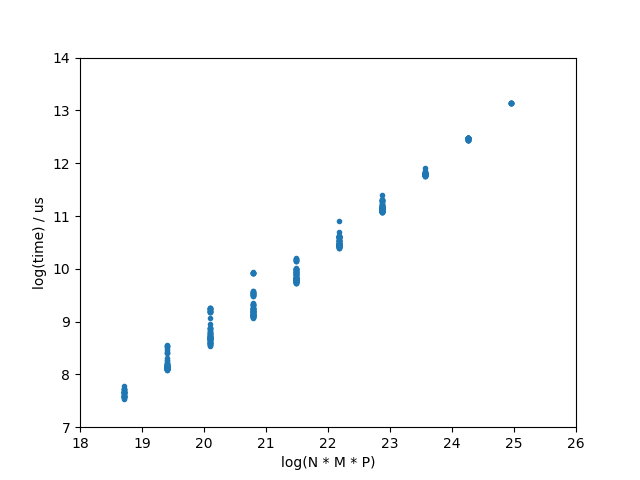
\includegraphics[width=0.8\textwidth]{figures/matmul_cpu_nmp.png}
        \caption{CPU矩阵乘法的性能数据(参数为$N \times M \times P $)}
        \label{fig:matmul_cpu_nmp}
    \end{figure}
    
    \begin{figure}[!htbp]
        \centering
        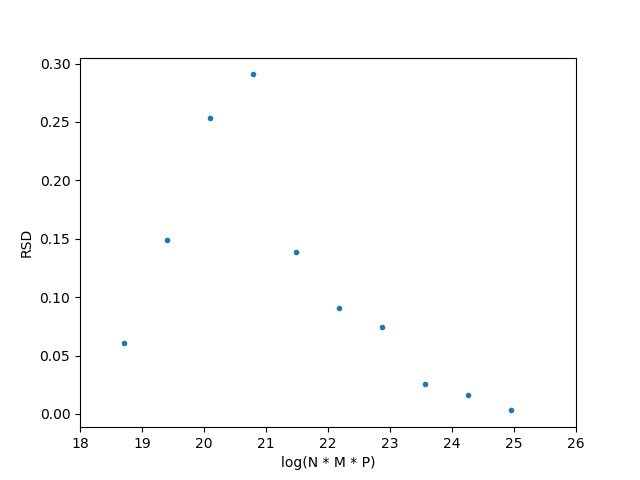
\includegraphics[width=0.8\textwidth]{figures/matmul_cpu_nmp_rsd.png}
        \caption{CPU矩阵乘法的相对标准偏差数据(参数为$ N \times M \times P $)}
        \label{fig:matmul_cpu_nmp_rsd}
    \end{figure}
    
    接下来我们考虑\ref{ssec:view_matmul}中提到的矩阵乘法计算过程,我们选取$ N \times M $和$ P $作为参数,这时我们发现数据相对$ N \times M $和$ P $都保持了比较好的正比例关系,同时,在固定取值的情况下,相对标准偏差低于0.1,可以满足我们的预测需求。因此,在CPU上最终的矩阵乘法性能模型采用$ N \times M $和$ P $作为参数,对性能数据进行线性插值。
    
    \begin{figure}[!htbp]
        \centering
        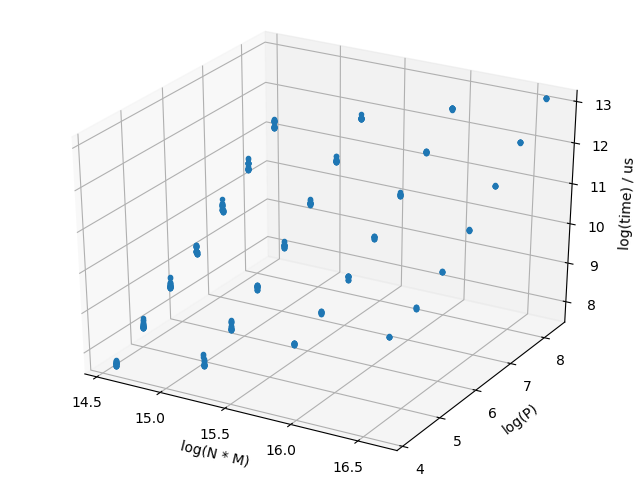
\includegraphics[width=0.8\textwidth]{figures/matmul_cpu_nm_p.png}
        \caption{CPU矩阵乘法的性能数据(参数为$N \times M $和$ P $)}
        \label{fig:matmul_cpu_nm_p}
    \end{figure}

    \begin{figure}[!htbp]
        \centering
        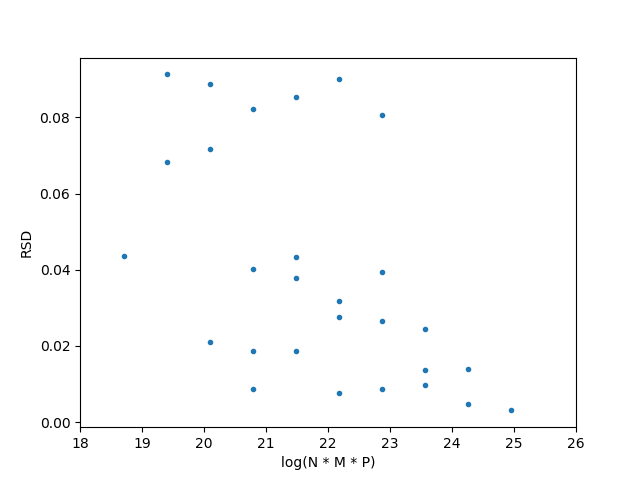
\includegraphics[width=0.8\textwidth]{figures/matmul_cpu_nm_p_rsd.png}
        \caption{CPU矩阵乘法的相对标准偏差数据(参数为$ N \times M $和$ P $)}
        \label{fig:matmul_cpu_nm_p_rsd}
    \end{figure}

    下面我们来对GPU数据进行建模。首先我们观察以$ N \times M \times P $为参数的数据,如图\ref{fig:matmul_gpu_nmp}所示。我们可以发现,在$ N \times M \times P $取值较大的时候,性能变化较少,而且很符合正比例函数。但是在取值较小的时候关系不明显,而且变化较大。
    
    我们考虑GPU计算矩阵乘法的过程,$ M \times N $代表线程数量,而GPU中线程数量和CPU相比大很多,以我们的实验平台V100为例,V100单卡支持线程数为5120,因此,在$ N \times M$规模不同的时候,会有不同的性能模型。
    
    \begin{figure}[!htbp]
        \centering
        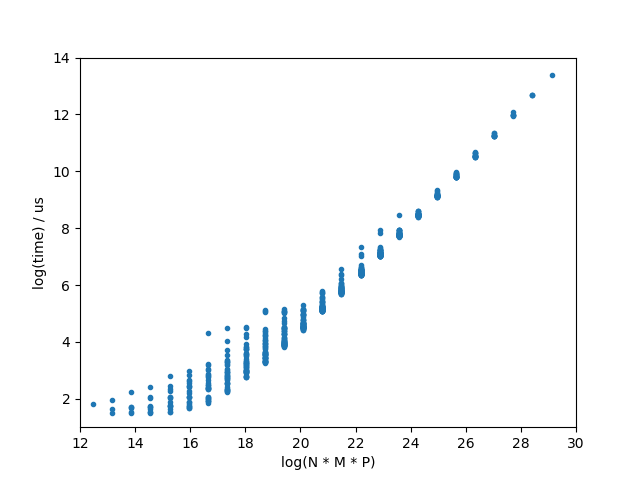
\includegraphics[width=0.8\textwidth]{figures/matmul_gpu_nmp.png}
        \caption{GPU矩阵乘法的性能数据(参数为$N \times M \times P $)}
        \label{fig:matmul_gpu_nmp}
    \end{figure}

    \begin{figure}[!htbp]
        \centering
        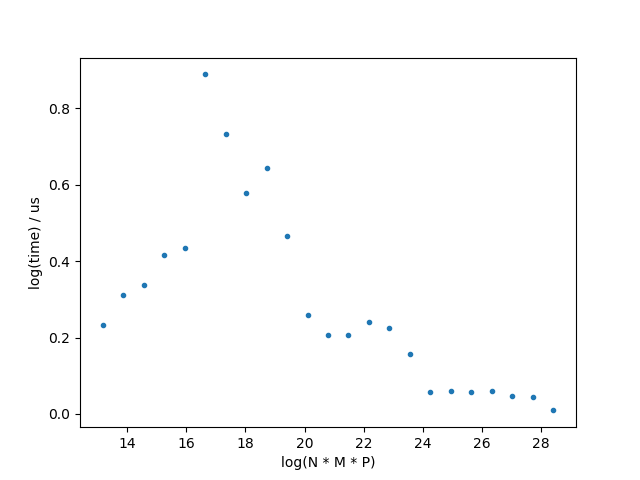
\includegraphics[width=0.8\textwidth]{figures/matmul_gpu_nmp_rsd.png}
        \caption{GPU矩阵乘法的相对标准偏差数据(参数为$ N \times M \times P $)}
        \label{fig:matmul_gpu_nmp_rsd}
    \end{figure}
    
    再卷积神经网络中,全连接层一般规模比较大,因此我们优先对规模较大的矩阵进行处理,
    因为在卷积神经网络中,一般全连接层规模较大,因此我们先考虑大规模的情况。我们把$ N $、$ M $规模限制到128以上,性能数据如图\ref{fig:matmul_gpu_nmp_big}所示,我们可以看出,无论是数据的线性程度还是数据的变化范围都有了很大的提升。图\ref{fig:matmul_gpu_nmp_rsd_big}指出,从相对标准偏差值来看,相较图\ref{fig:matmul_gpu_nmp_rsd},在矩阵规模较大的时候,使用$ N \times M \times P $为参数,就可以达到比较好的预测效果了。因此,我们将输入规模以$128 \times 128$作为分界线,使用两个模型,小模型使用$ N $、$ M $、$ P $三个参数建模,而大模型使用$ N \times M \times P $作为参数建模,就能得到比较准确的预测结果了。

    \begin{figure}[!htbp]
        \centering
        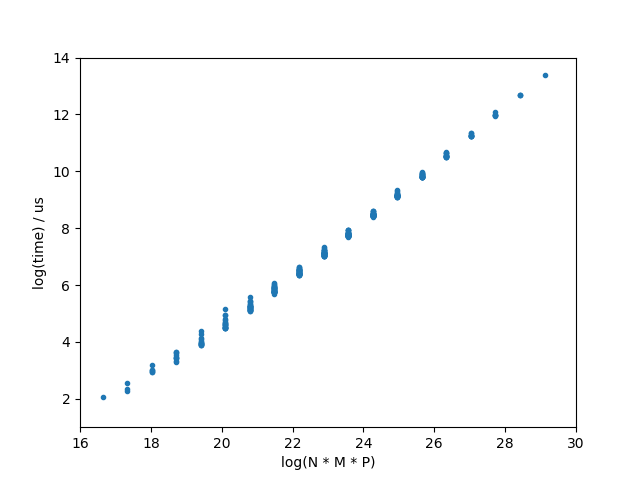
\includegraphics[width=0.8\textwidth]{figures/matmul_gpu_nmp_big.png}
        \caption{GPU矩阵乘法的性能数据(参数为$N \times M \times P $,$ N $、$ M $、$ P $取值128以上)}
        \label{fig:matmul_gpu_nmp_big}
    \end{figure}

    \begin{figure}[!htbp]
        \centering
        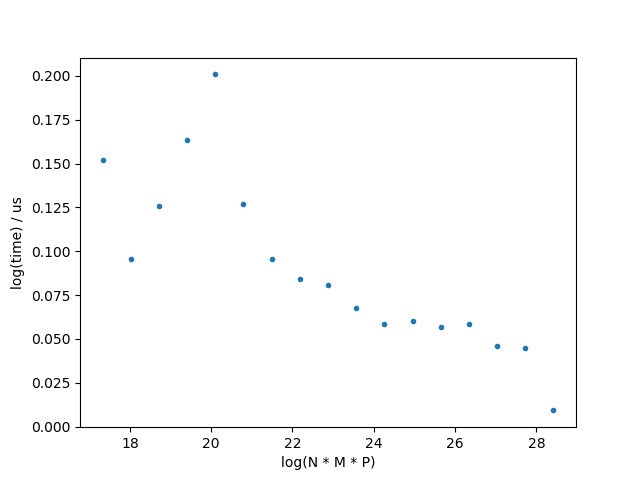
\includegraphics[width=0.8\textwidth]{figures/matmul_gpu_nmp_rsd_big.png}
        \caption{GPU矩阵乘法的相对标准偏差数据(参数为$ N \times M \times P $,$ N $、$ M $、$ P $取值128以上)}
        \label{fig:matmul_gpu_nmp_rsd_big}
    \end{figure}

\subsection{二维卷积}
\label{ssec:impl_conv}
    二维卷积操作的运算包含6个参数,图片数量($ B $)、图片尺寸($ W \times H $)、卷积核尺寸($ W_K \times H_K $)、输入通道数($ C_{in} $)、输出通道数($ C_{out} $)、步长($ W_S \times H_S $)。因此我们针对以上六个参数进行性能测试,得到在CPU和GPU上的性能数据。

    首先考虑CPU的情况,我们使用$ B \times W \times H \times W_K \times W_H \times W_S^{-1} \times H_S^{-1} \times C_{in} \times C_{out} $作为参数,得到性能数据如图\ref{fig:conv_cpu}所示。我们看到,参数取值相同时,数据变化范围较大,不能够直接使用。而我们经过观察,可以看出,性能数据图中隐约显示出4条平行的直线。而数据中取值有4种的参数仅有$ C_{in} $和$ C_{out} $,因此,我们取参数$ B \times W \times H \times W_K \times W_H \times W_S^{-1} \times H_S^{-1} \times C_{in} $和$ B \times W \times H \times W_K \times W_H \times W_S^{-1} \times H_S^{-1} \times C_{out} $。我们发现,当我们仅选$ B \times W \times H \times W_K \times W_H \times W_S^{-1} \times H_S^{-1} \times C_{in}  $为参数时图像变得较为清晰,如图\ref{fig:conv_cpu_fix0}所示。但依然有大量点不符合正比例函数。
    
    在二维卷积操作中,如果卷积核仅为一个点,那么二维卷积运算会退化为矩阵和数字的乘法,此时不会调用二维卷积操作的函数,因此,我们去除这类点,得到性能数据如图\ref{fig:conv_cpu_fix1}所示,此时平均相对标准偏差为0.18可以满足我们的需求。

    \begin{figure}[!htbp]
        \centering
        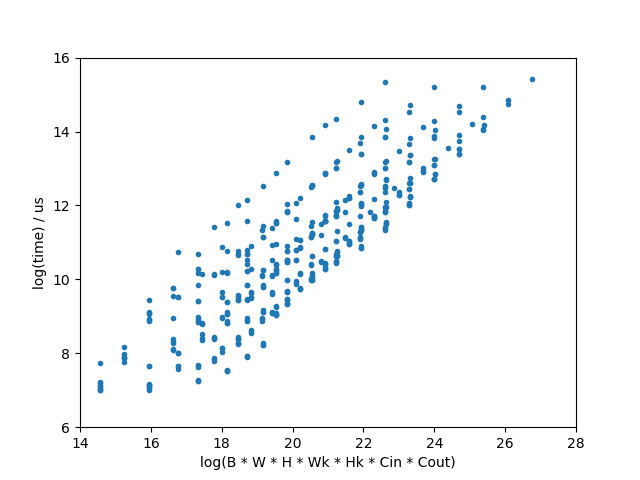
\includegraphics[width=0.8\textwidth]{figures/conv_cpu.png}
        \caption{CPU二维卷积的性能数据(参数为用$ B \times W \times H \times W_K \times W_H \times W_S^{-1} \times H_S^{-1} \times C_{in} \times C_{out} $)}
        \label{fig:conv_cpu}
    \end{figure}

    \begin{figure}[!htbp]
        \centering
        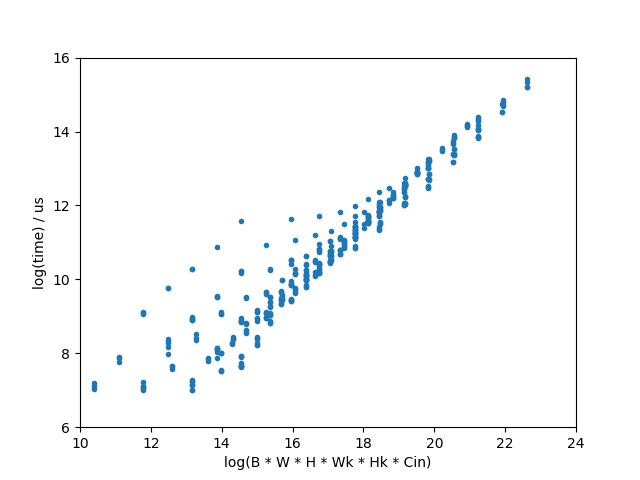
\includegraphics[width=0.8\textwidth]{figures/conv_cpu_fix0.png}
        \caption{CPU二维卷积的性能数据(参数为$ B \times W \times H \times W_K \times W_H \times W_S^{-1} \times H_S^{-1} \times C_{in}  $)}
        \label{fig:conv_cpu_fix0}
    \end{figure}

    \begin{figure}[!htbp]
        \centering
        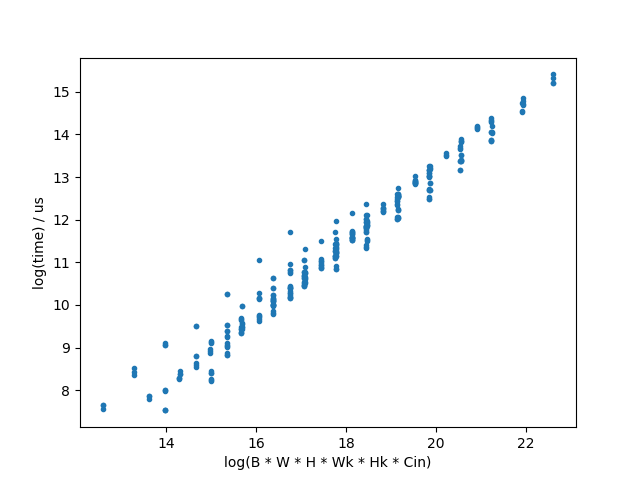
\includegraphics[width=0.8\textwidth]{figures/conv_cpu_fix1.png}
        \caption{CPU二维卷积的性能数据(参数为$ B \times W \times H \times W_K \times W_H \times W_S^{-1} \times H_S^{-1} \times C_{in}  $,去除卷积核大小为1的情况)}
        \label{fig:conv_cpu_fix1}
    \end{figure}

    在GPU上,二维卷积操作会采用不同的优化方式,调用不同的CuBlas或CuDNN函数,这时数据规律并不直观,因此我们无法直接降低参数个数,只能直接对数据进行插值。
    
    \begin{figure}[!htbp]
        \centering
        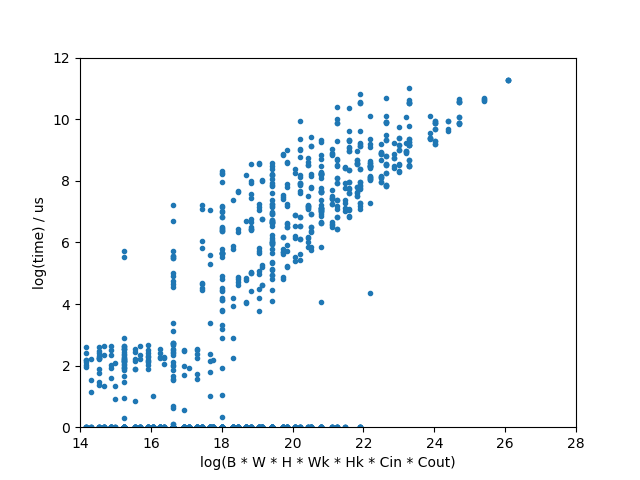
\includegraphics[width=0.8\textwidth]{figures/conv_gpu.png}
        \caption{GPU二维卷积的性能数据(参数为$ B \times I^2 \times K^2 \times C_{in} \times C_{out} $)}
        \label{fig:conv_gpu}
    \end{figure}
    
\subsection{局部响应归一化}
    局部相应归一化的输入是一个四维张量。其中前三维的乘积我们作为参数$ M $,第四维作为参数$ N $,深度半径作为参数$ R $。

    在CPU上,我们以$ M \times N $为参数,这时局部响应归一化的性能数据如图\ref{fig:lrn_cpu}所示,此时的平均相对标准偏差为0.15可以满足我们的需求。
    
    \begin{figure}[!htbp]
        \centering
        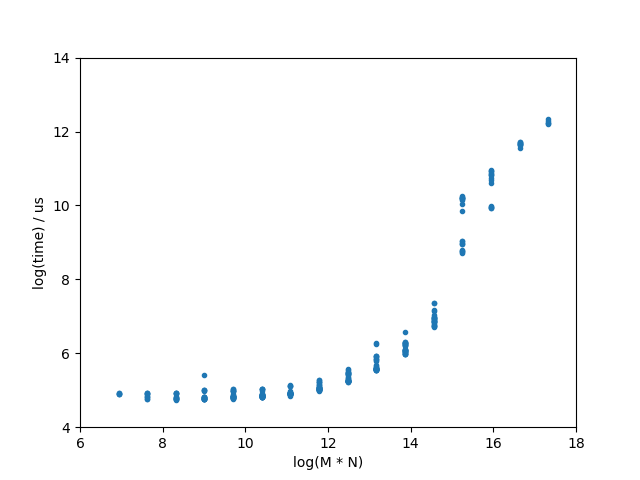
\includegraphics[width=0.8\textwidth]{figures/lrn_cpu.png}
        \caption{CPU局部响应归一化的性能数据(参数为$ M \times N $)}
        \label{fig:lrn_cpu}
    \end{figure}

    在GPU上,局部响应归一化函数的性能数据如图\ref{fig:lrn_gpu}所示,此时平均相对标准偏差为0.14,也满足我们的需求。

    \begin{figure}[!htbp]
        \centering
        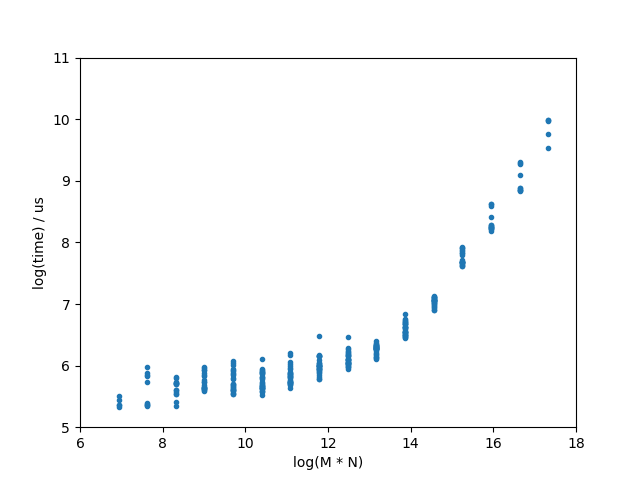
\includegraphics[width=0.8\textwidth]{figures/lrn_gpu.png}
        \caption{GPU局部响应归一化的性能数据(参数为$ M \times N $)}
        \label{fig:lrn_gpu}
    \end{figure}

\subsection{数据传输}
    在使用GPU的情况下,我们还需要考虑CPU和GPU之间,GPU和GPU之间的数据传输问题,即对cuMemcpyDtoH, cuMemcpyHtoD, cuMemcpyPtoP进行建模。
    我们默认TensorFlow能够占用整个机器的所有资源,不会和其他应用抢占。这时不考虑函数调用带来的时间,那么我们的数据传输能够占用所有的带宽。因此,cuMemcpyDtoH和cuMemcpyHtoD的执行时间应该为数据传输量除以PCIE带宽。而cuMemcpyPtoP的执行时间为数据传输量除以NVLink带宽。

    以我们的实验平台为例,PCIE带宽为32GB/s。我们直接建模。NVLink带宽为900GB/s,运行时间过快,不会对我们的模型造成影响,因此省略。

\subsection{数据修正}
    之前讨论的性能模型中,都存在不很符合我们预测模型的数据点,对这类数据点,我们采用提前存储的方式进行处理。针对之前测试中离模型相差过远的数据点,我们测试它周围一定范围的数据。测试数据落在这个范围内时,我们使用这一范围内的数据点进行插值,作为最终的预测结果,从而避免之前建立的模型精度不足的情况。
    
    另外,由于常用的卷积神经网络中使用的卷积操作规模都比较相似,因此,我们也可以将常用的操作参数也作为特殊节点进行测试,这样在测试的时候,我们就可以更容易地得到准确的性能数据。在后续测试中,为了保证实验的可信性,我们没有在实验使用的版本中部署这个优化。

\section{调度模拟}
    调度模拟部分主要处理四部分工作:
    \begin{itemize}
        \setlength{\itemindent}{1em}
        \item {\bfseries 生成}:将用户输入的TensorFlow代码转化为数据流图的形式。
        \item {\bfseries 剪枝}:根据输入输出列表对数据流图进行剪枝,得到最小依赖集。
        \item {\bfseries 预测}:根据设定好的配置代入性能模型数据,预测性能。
        \item {\bfseries 模拟}:动态模拟模型运行状况。
    \end{itemize}
    
    下面分别就四部分工作的实现进行讲解。

\subsection{生成}
    数据流图的生成,我们通过直接调用TensorFlow接口的方式进行。用户正常编写TensorFlow代码,我们创建会话,获得计算图保存为JSON格式,作为下一部分的输入。

    接下来对计算图进行处理,首先根据JSON中的信息将图重新组织为点集的形式,每个点保存名称、输入、输出、操作类型等信息,再将用户输入的规模信息作为参数保存在相应节点上。最后将部分操作扩展为子图,即完成图的生成。

\subsection{剪枝}
    剪枝操作是为了获得最小依赖集,TensorFlow中使用DFS进行剪枝。在我们的系统中,结合我们的存储方式,我们使用BFS实现,从输出点开始,反向搜索依赖点,最终没有被覆盖的点直接删除。

    实际正常定义的深度神经网络任务中,不存在冗余节点,因此这一步并不能有效减少预测信息内容。

\subsection{预测}
    预测部分将每个操作需要的计算时间填入到数据流图中对应节点的信息中。由于操作执行的硬件信息被存储到了数据流图的节点中,因此这一步只需要遍历数据流图,查询性能模型,再写入数据即可。

\subsection{模拟}
    在得到准备好的数据流图后,我们进行调度模拟,以求尽量还原TensorFlow的动态调度过程。

    考虑到在二维卷积操作在CPU上可能存在的不能占满所有线程的情况。我们在模拟过程中还需要考虑每个任务在当前运行状态下,实际能占用的CPU计算资源比例。

    我们首先将输入节点加入待运行队列中,在每一轮运行时,我们根据资源使用情况,尽量将新的节点加入运行,每一轮运行的时候根据当前操作占用的资源调整每个操作的剩余时间,如原本操作占用所有CPU资源,还需要运行400ms,那么加入一个新的操作后,该操作只能占用50\%的资源,因此剩余时间变化为800ms。选择完成时间最短的操作,更新整体完成时间,再进入下一轮迭代。重复这一个过程,我们就可以比较准确地模拟TensorFlow中操作的动态调度过程了。

    实际使用中,由于性能模型存在误差,因此不能保证调度过程和TensorFlow的调度过程完全相同。但是考虑到一般的卷积神经网络是分层的,层内还有同步,因此我们的预测模式在调度层面通常不会带来很大的误差,这一点在\ref{cha:eval}中会详细介绍。
